\chapter{DNA sequence classification} \label{sec:dna_sequences}

\section{DNA sequences} \label{subsec:what_are_dna_sequences}

Deoxyribonucleic acid (DNA) is composed of a linear string of nucleotides, or bases, which are referred to by their chemical names' first letters: \gls{A}, \gls{T}, \gls{C}, and \gls{G}. 

DNA sequencing is the technique of finding the order of the four bases. Scientists can determine the type of genetic information carried in a DNA segment by examining the sequence. Furthermore, and more significantly, sequencing data can reveal mutations in a gene that could lead to illness, by comparing a healthy and a mutated sequence~\cite{2020DNASheet}.

The four chemical bases of the DNA double helix always connect with the same partner to produce "base pairs". \gls{A} is always paired with \gls{T}, while \gls{C} is always paired with \gls{G} (Figure~\ref{fig:dna}). This pairing explains the technique by which DNA molecules are copied when cells divide, as well as the methods used in most DNA sequencing research. The human \gls{genome} is made up of around 3 billion base pairs, which carry the instructions for creating and maintaining a human person~\cite{2020DNASheet}.

\begin{figure}[htbp]
    \centering
    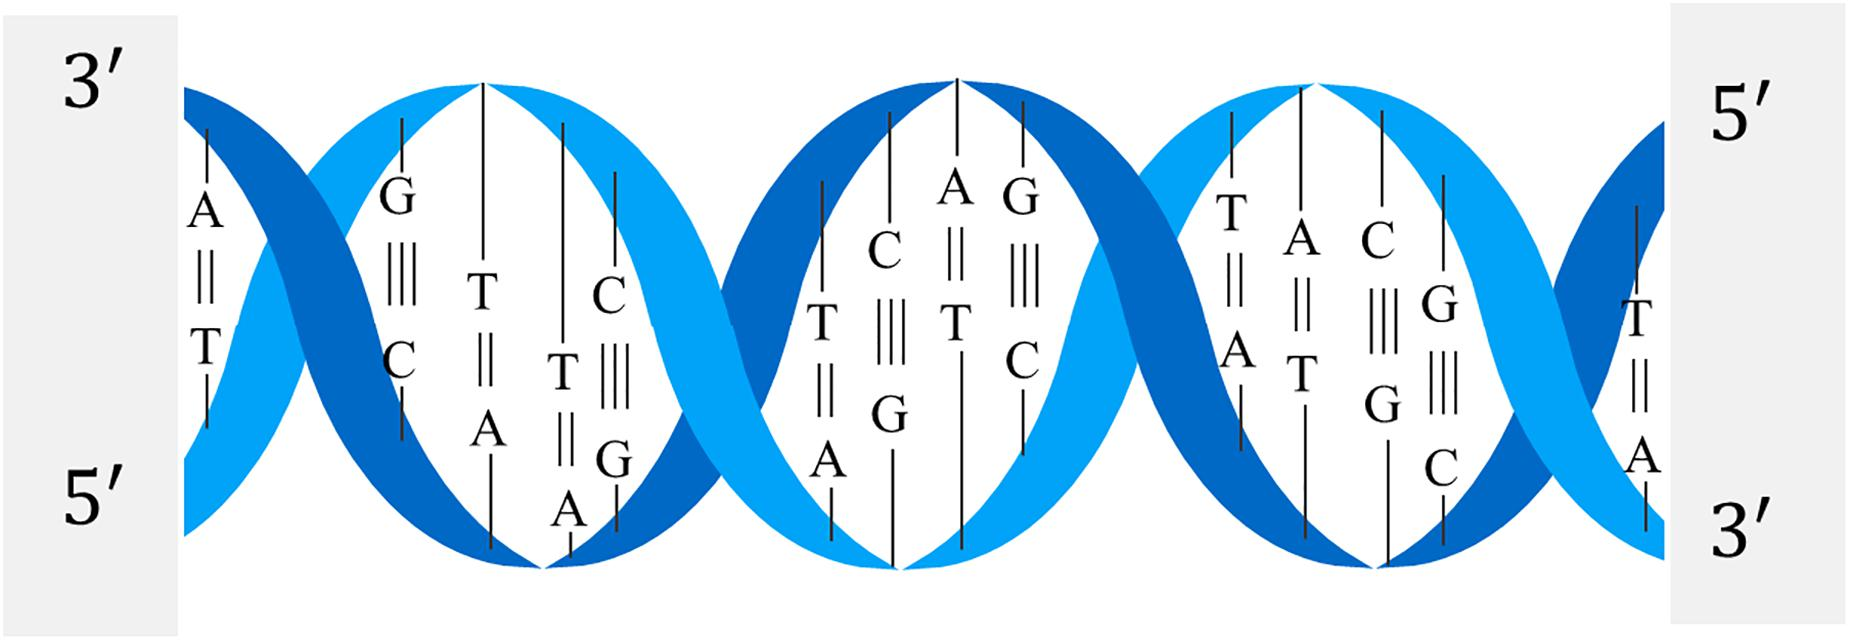
\includegraphics[width=0.5\linewidth]{Chapters/Figures/dna.jpg}
    \caption{Double helix of DNA~\cite{Yang2020ReviewDNA}}
    \label{fig:dna}
\end{figure}

Since the Human Genome Project's completition~\cite{TheProject}, technological advancements and automation have made it possible for individual genes to be sequenced on a regular basis, by reducing the amount of time it takes to perform the sequencing and also reducing its cost. Some labs can sequence over 100,000 billion bases per year, and a few thousand dollars is enough to sequence an entire \gls{genome}~\cite{2020DNASheet}. 

\section{DNA sequence classification ML tradicional}

%Descriptors 
%Algorithms 

\section{DNA sequence classification DL}
